\subsubsection{Gestione ad alto livello della CFA}
Avendo introdotto due molteplici tipi di codice eseguibile, ovvero le definizioni di funzioni e gli overload generati implicitamente 
tramite \textit{Common Features Adoption} (CFA), allora è stato necessario introdurre un layer di astrazione rispetto ad essi 
tramite la classe \texttt{CallableCodeBlock}. Tale classe è super-tipo di entrambe secondo la definizione di super-tipo 
data nell'approfondimento dei design pattern in C++. \\

\begin{figure}[h]
    \centering
        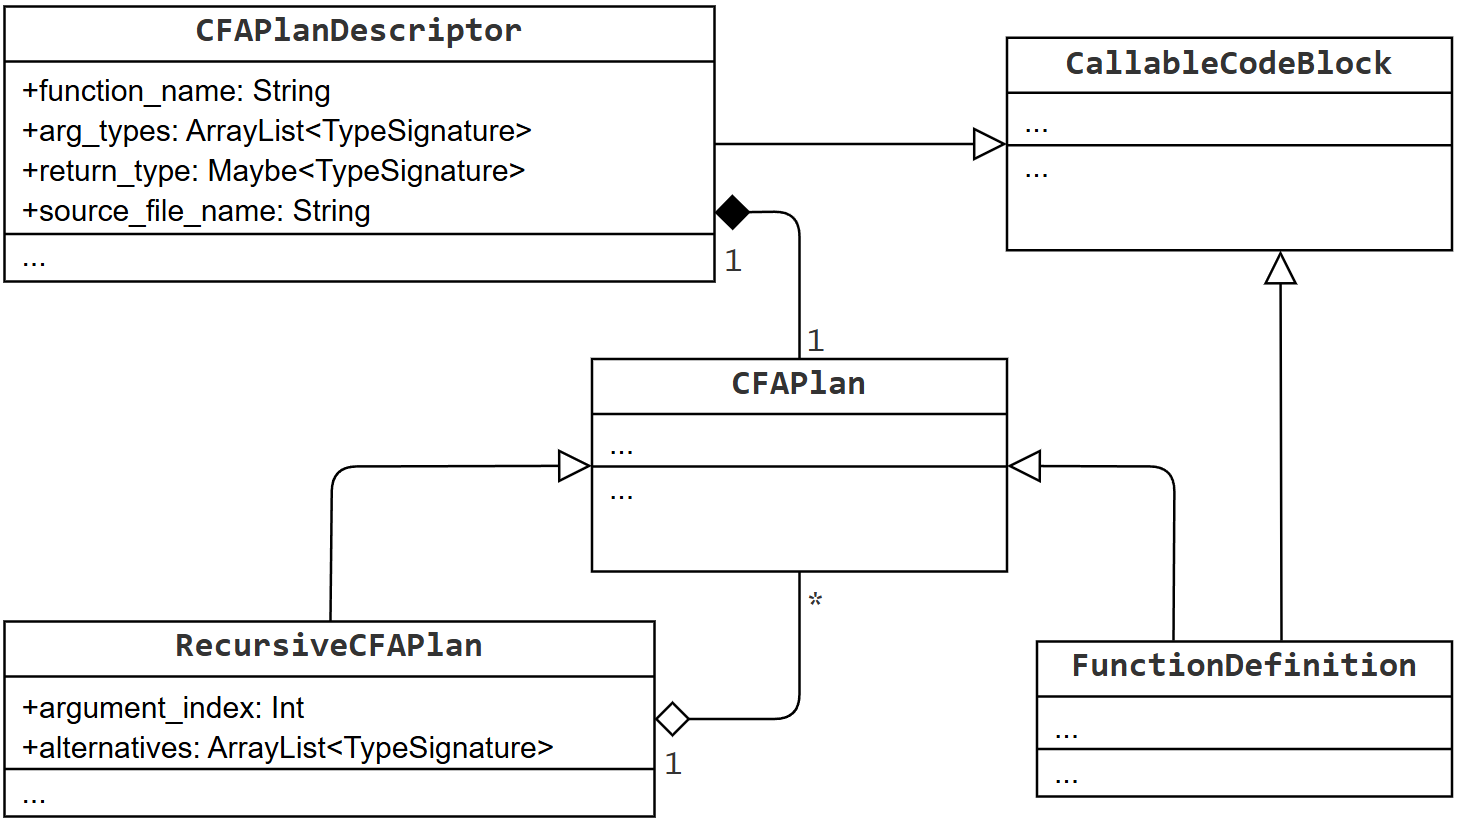
\includegraphics[width=1\textwidth]{../../Assets/CFA_UML.png}
    \caption{
        \centering
        Diagramma UML semplificato delle relazioni tra le classi che 
        modellano blocchi di codice eseguibile: definizioni di funzioni e overload CFA}
\end{figure}
\vspace{0.5cm}

Un \texttt{CFAPlanDescriptor} è un oggetto che modella la radice di un albero decisionale, di cui ogni foglia è una \texttt{FunctionDefinition}, 
mentre ogni nodo non-foglia è un \texttt{RecursiveCFAPlan} che codifica le possibili scelte durante il runtime-dispatch. \\

Si considerino infatti le seguenti definizioni di funzioni (saranno fornite solo le firme): \\

\vspace{0.5cm}
\begin{lstlisting}[frame=single]
func max(x : Int,   y : Int)   -> Int   { /* ... */ }
func max(x : Float, y : Float) -> Float { /* ... */ }
func max(x : Float, y : Int)   -> Float { /* ... */ }
func max(x : Int,   y : Float) -> Float { /* ... */ }
\end{lstlisting}

\newpage

Una chiamata alla funzione \texttt{max} con entrambi gli argomenti di tipo dichiarato \texttt{Int|Float} sarebbe risolta 
generando un'overload CFA, il quale sarebbe modellato come: \\

\begin{figure}[h]
    \centering
        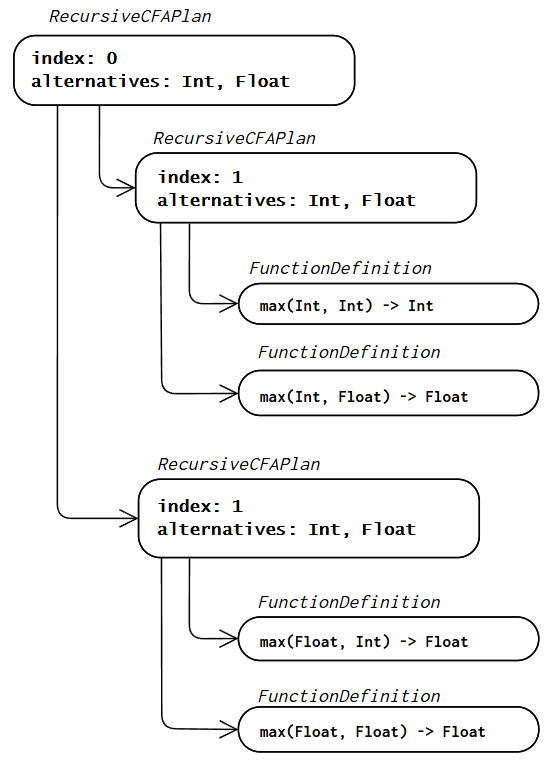
\includegraphics[height=0.9\textwidth]{../../Assets/CFA_ML.png}
    \caption{
        \centering
        Memory-layout di un albero CFA per una chiamata alla funzione
        \texttt{max} con argomenti di tipo \texttt{Int|Float}
    }
\end{figure}
\vspace{0.5cm}

Tale albero rappresenta in tutto e per tutto un processo decisionale da effettuarsi a tempo di esecuzione 
dove per ogni nodo \texttt{RecursiveCFAPlan} ci si chiede quale sia il tipo concreto dell'argomento 
all'indice corrente, e si procede navigando sul figlio corrispondente. Arrivati su di una foglia, si chiama 
la funzione corrispondente. \\

\newpage

La generazione di un \texttt{CFAPlanDescriptor} è responsabilità della classe \texttt{CFAPlanGenerationEngine}, 
la quale procede secondo l'algoritmo ora illustrato: \\ 

(dato che la generazione di un \texttt{CFAPlan} è esosa di risorse, la classe \texttt{CFAPlanGenerationEngine} 
utilizza una cache chiave/valore con chiavi stringhe costruite similmente a quanto visto per \texttt{FunctionDefinitionsRegister}): \\

\vspace{0.5cm}
\begin{lstlisting}[frame=single]
CFAPlanGenerationEngine.generate_plan(func_call, arg_types): 
    key = get_cache_fast_search_key(func_call, arg_types)
    if (cache[key] != nil):
        return cache[key]
    cfa_plan = generate_plan(
        function_call, 
        arg_types, 
        0 // <--- start from the first argument
    )
    cache[key] = cfa_plan
    return cfa_plan
\end{lstlisting}
\vspace{0.5cm}

\vspace{0.5cm}
\begin{lstlisting}[frame=single]
CFAPlanGenerationEngine.generate_plan(func_call, arg_types, index): 
    if (index >= function_call.arguments.size()):
        return nil
    fdef = search_function_definition(func_call, arg_types)
    if (fdef != nil):
        return fdef 
    if (!function_call.arguments[index].is_union()):
        return generate_plan(
            function_call, 
            arg_types, 
            index + 1
        )
    plan = RecursiveCFAPlan()
    current = function_call.arguments[index].get_union()
    plan.alternatives = current.get_alternatives()
    for alternative in plan.alternatives:
        new_arg_types = arg_types
        new_arg_types[index] = alternative
        plan.children.append(
            generate_plan(
                function_call, 
                new_arg_types, 
                index + 1
            )
        )
\end{lstlisting}
\vspace{0.5cm}